\documentclass[notitlepage]{report}

\author{Cronqvist, Fredrik \and Larsson, Sebastian \and Stenberg, Victor \and S\"{a}ll, Martin}
\date{\today}
\title{League of Legends learning analysis}

\usepackage{graphicx}

\begin{document}
\maketitle

\begin{abstract}
[Placeholder text]
\end{abstract}

\begingroup
\chapter*{Preface}
We would like to thank Emelie and Pontysius the Great for participating in our experiment.

\let\clearpage\relax

\tableofcontents
\endgroup

\chapter{Introduction}
This report takes on some questions about where players playing the computer game League of Legends with different levels of experience focus on the screen, what their priorities are during gameplay and how long they take to finish a round in the game. In hopes of discovering a trend six participants have been eye-tracked while playing one round in the game. The participants will be referred to P1, P2, … and P6, in order of experience with the game, where P1 has the least experience and P6 has the most.

\section{League of Legends}
League of Legends (LoL) is multiplayer online battle arena (moba) game. By default two teams of five players each, participate with the goal of destroying the base of the opposing team. Each player controls a hero with unique abilities on the battlefield trying to achieve this goal.

The map is split into three different `lanes' where most of the combat occurs, separated by a `jungle', a traversable area with less visibility and many twists and turns. Because of this layout, keeping track of the players on one's own team as well as opponents is important to successful tactics. This is primarily accomplished through the use of a mini-map, a small area in the lower right corner showing a top down view of the area with icons for each players, colored by team.

As the game progresses, each player accumulates gold, the in-game currency, which is meant to be spent in a shop in each team's base to buy items that improves the player's stats for the duration of the game.

\section{Hypothesis and questions}
There is a distinct difference between how new players and experienced players look at the screen to attain information.

\begin{itemize}
\item Does the new players find the shop?
\item Do new players lay less time on the mini-map then experienced players?
\item Are we able to improve the learning curve for new players and still keep the enjoyment for the experienced players?
\item Are new players available to find the shop?
\end{itemize}

\chapter{Analysis}
All of the data retrieved from the experiment are gaze plots and heat maps, every participant will have one of each. To make the analysis more accurate we sorted them into two separate groups, the inexperienced group (group 1) and the experienced group (group 2). P1, P2, P3 and P4, P5, P6 belongs to each group respectively. Each group have its group members’ gaze plots and heat maps combined into a single gaze plot and heat map to enhance the analysis.

\section{Group 1 analysis}
P1 and P2 have no experience with moba games and P3 has played about 10 hours. As for this groups’ heat map some data can be extracted. They have a great focus on the middle screen where there character are and some focus on the skills in the middle bottom of the screen.  They also lay much more time on the mini-map down to the right. Some of the places they don't look too much on are down to the left, on the character stats, items and how much gold they have. Also there was nearly no focus on info of the other teammates and the game stats.

\section{Group 2 analysis}

\begin{figure}[ht]
\begin{minipage}[b]{0.45\linewidth}
\centering
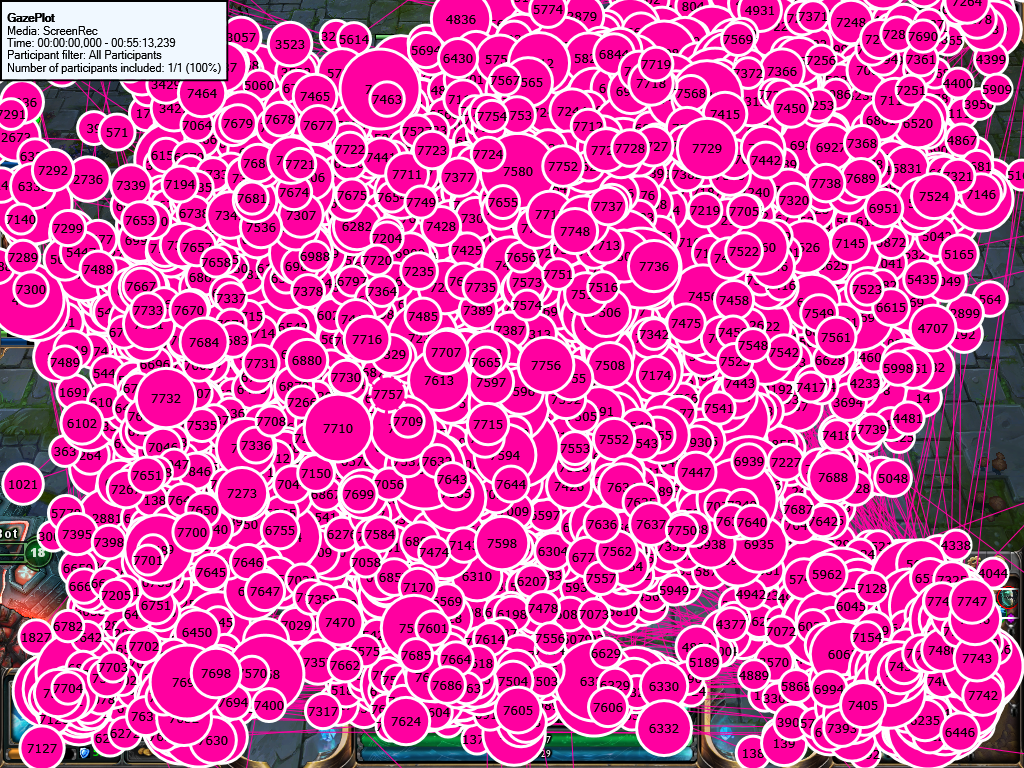
\includegraphics[width=\textwidth]{images/gazeplot/Emelie}
\caption{Gaze plot P1}
\label{gaze_eme}
\end{minipage}
\hspace{0.5cm}
\begin{minipage}[b]{0.45\linewidth}
\centering
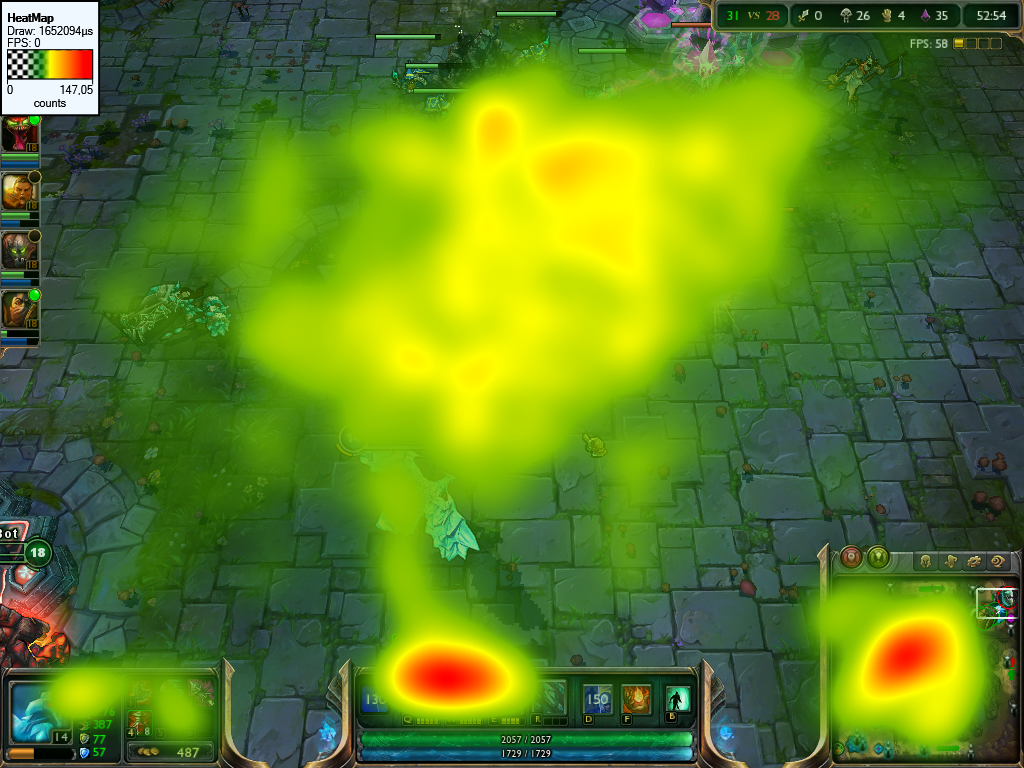
\includegraphics[width=\textwidth]{images/heatmap/Emelie}
\caption{Heat map P1}
\label{heat_eme}
\end{minipage}
\end{figure}

\begin{figure}[ht]
\begin{minipage}[b]{0.45\linewidth}
\centering
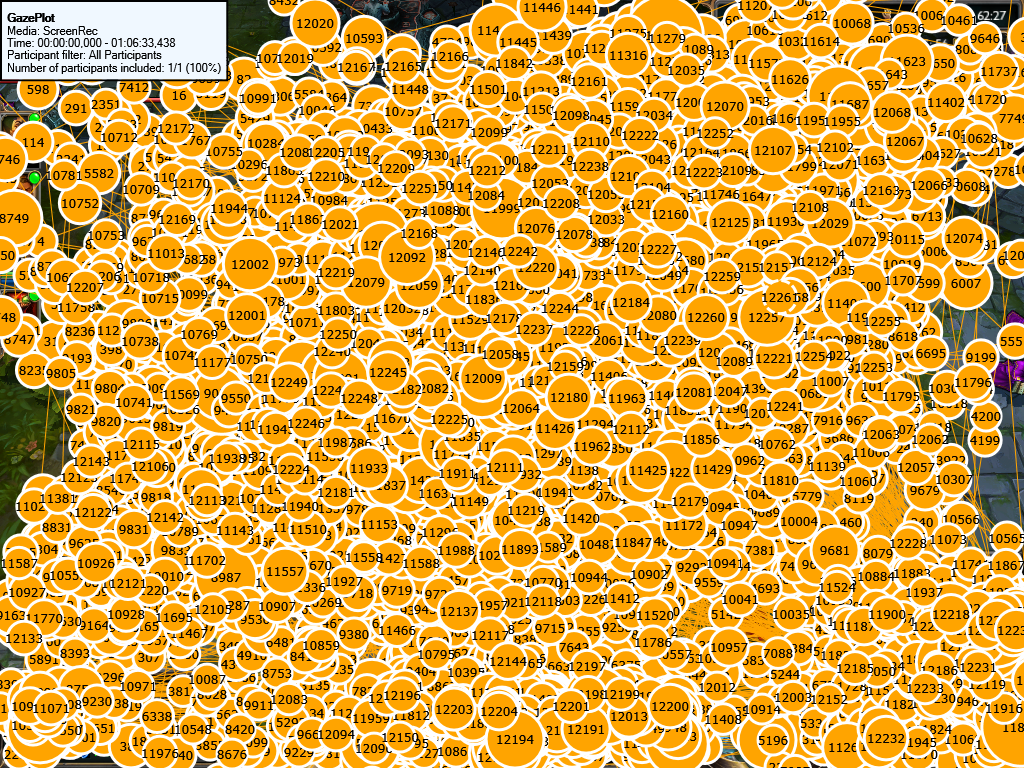
\includegraphics[width=\textwidth]{images/gazeplot/Pontus}
\caption{Gaze plot P2}
\label{gaze_pon}
\end{minipage}
\hspace{0.5cm}
\begin{minipage}[b]{0.45\linewidth}
\centering
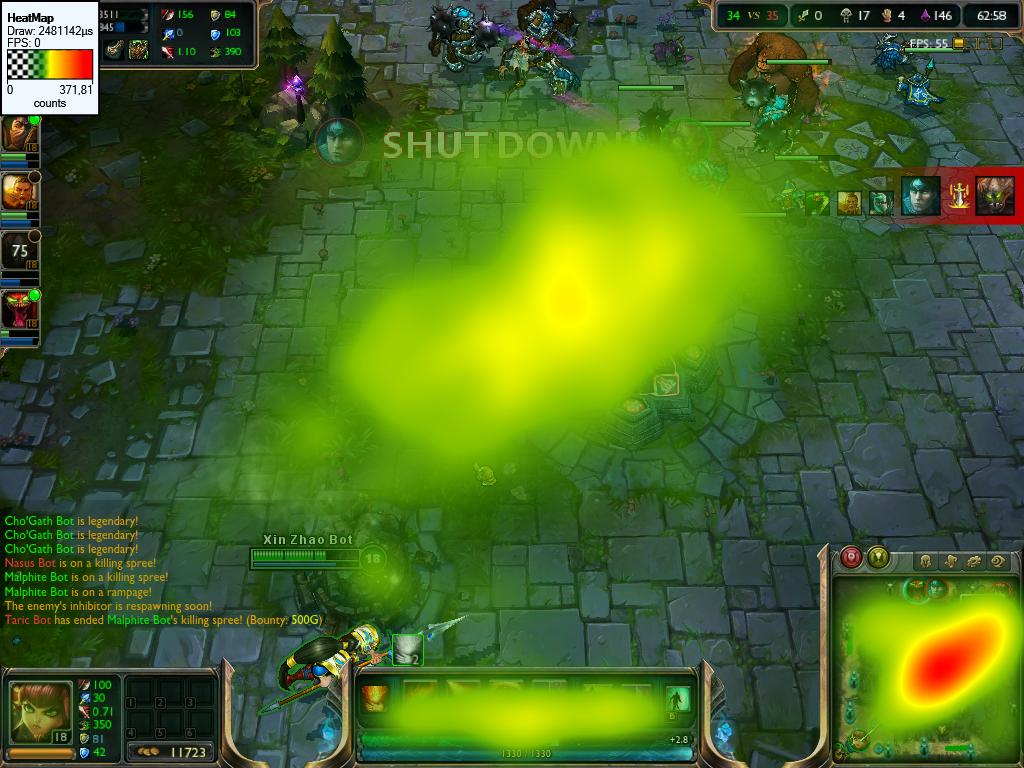
\includegraphics[width=\textwidth]{images/heatmap/Pontus}
\caption{Heat map P2}
\label{heat_pon}
\end{minipage}
\end{figure}

\begin{figure}[ht]
\begin{minipage}[b]{0.45\linewidth}
\centering
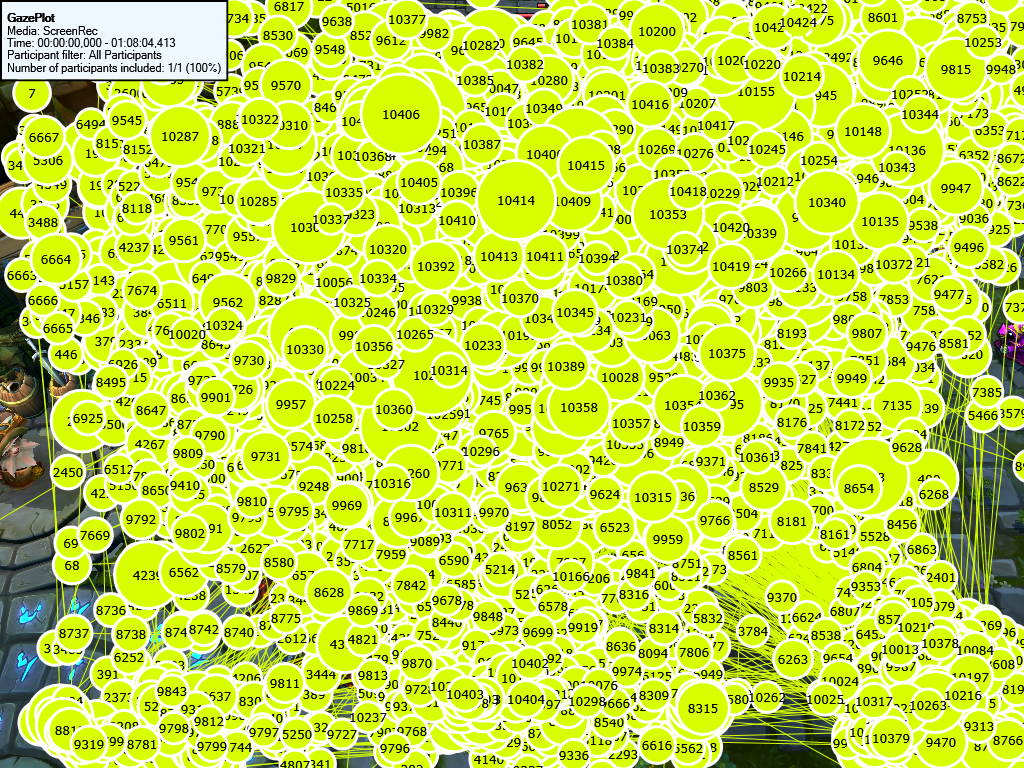
\includegraphics[width=\textwidth]{images/gazeplot/Sebastian}
\caption{Gaze plot P3}
\label{gaze_seb}
\end{minipage}
\hspace{0.5cm}
\begin{minipage}[b]{0.45\linewidth}
\centering
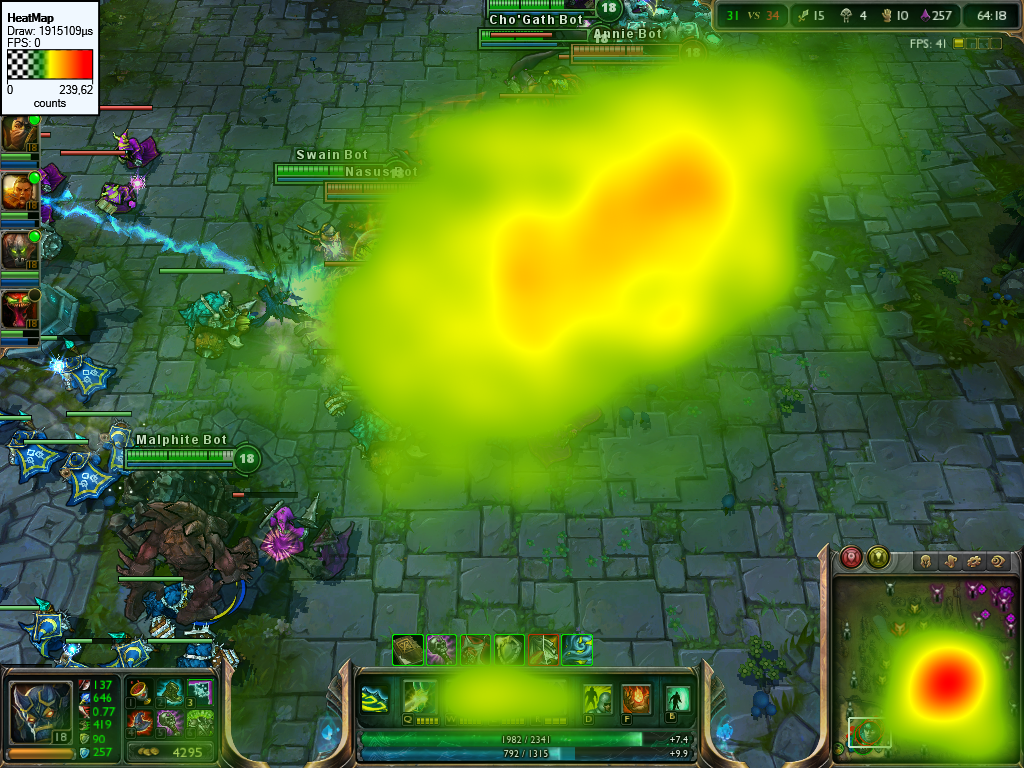
\includegraphics[width=\textwidth]{images/heatmap/Sebastian}
\caption{Heat map P3}
\label{heat_seb}
\end{minipage}
\end{figure}

\begin{figure}[ht]
\begin{minipage}[b]{0.45\linewidth}
\centering
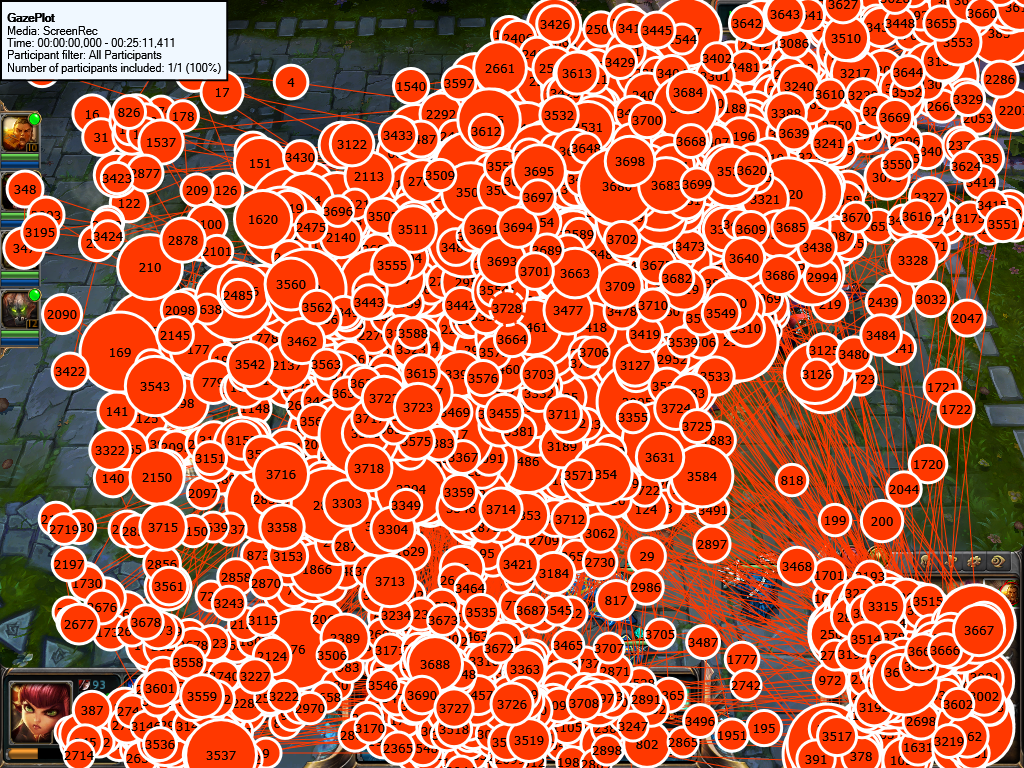
\includegraphics[width=\textwidth]{images/gazeplot/Victor}
\caption{Gaze plot P4}
\label{gaze_vic}
\end{minipage}
\hspace{0.5cm}
\begin{minipage}[b]{0.45\linewidth}
\centering
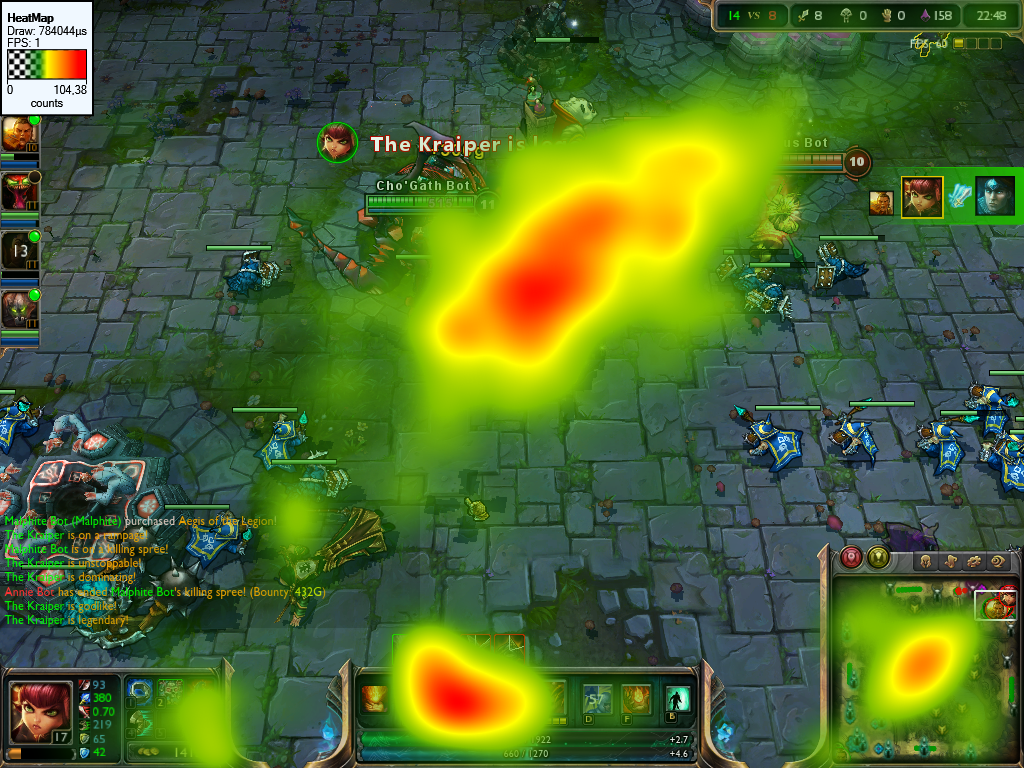
\includegraphics[width=\textwidth]{images/heatmap/Victor}
\caption{Heat map P4}
\label{heat_vic}
\end{minipage}
\end{figure}

\begin{figure}[ht]
\begin{minipage}[b]{0.45\linewidth}
\centering
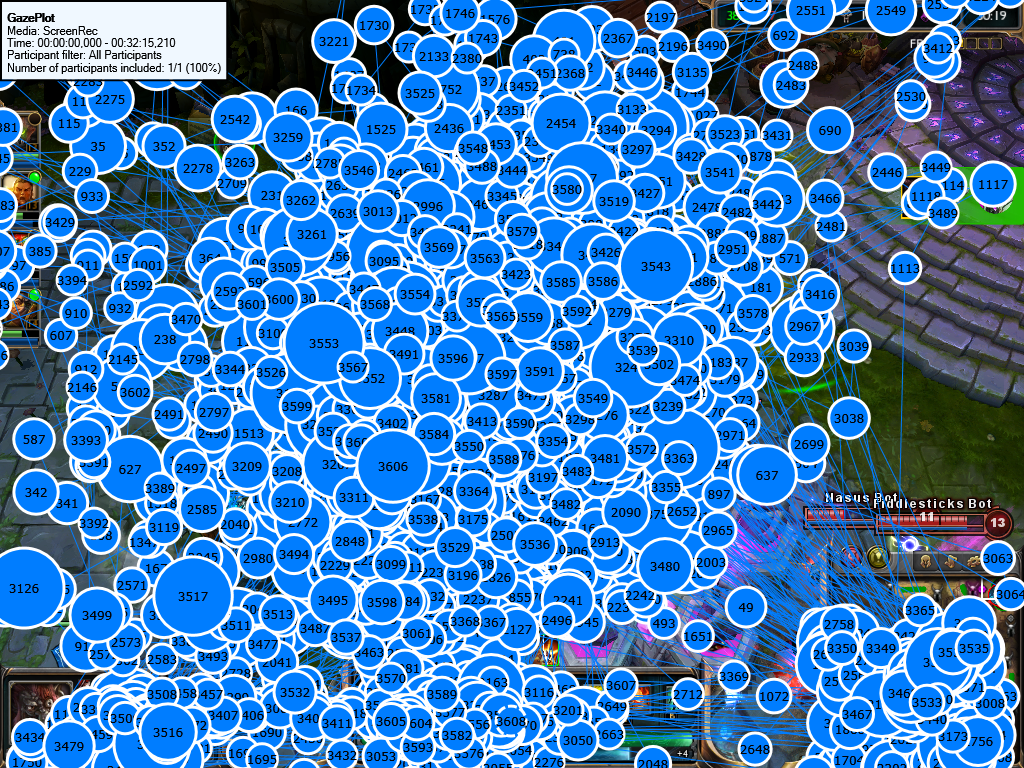
\includegraphics[width=\textwidth]{images/gazeplot/Fredrik}
\caption{Gaze plot P5}
\label{gaze_fre}
\end{minipage}
\hspace{0.5cm}
\begin{minipage}[b]{0.45\linewidth}
\centering
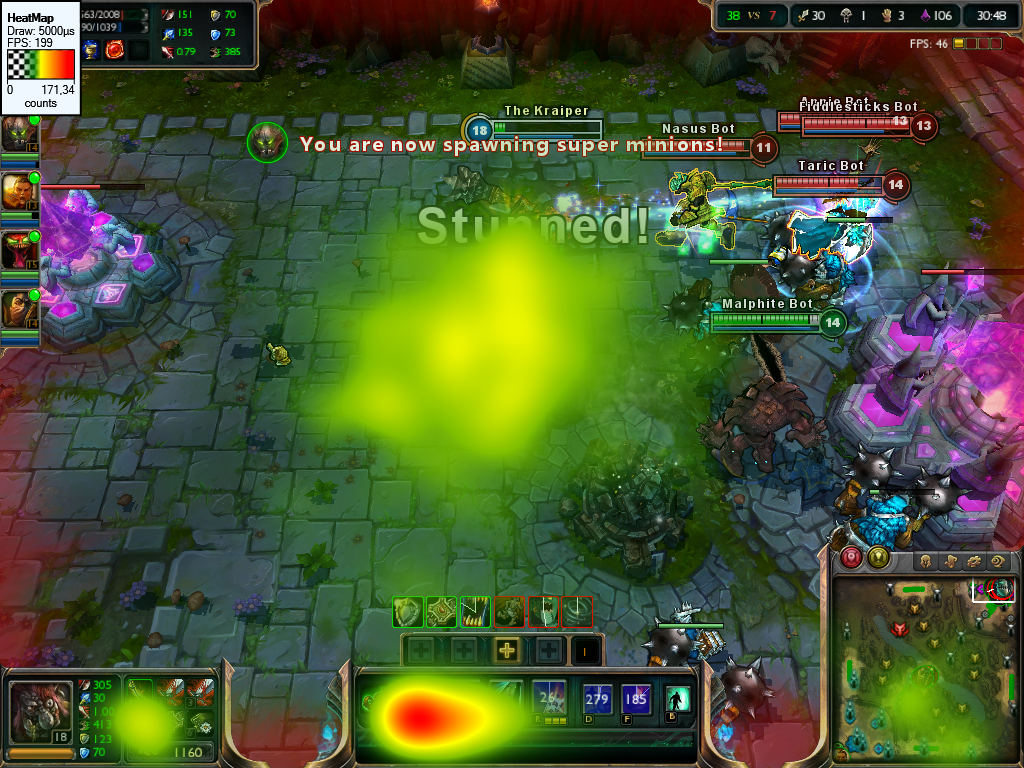
\includegraphics[width=\textwidth]{images/heatmap/Fredrik}
\caption{Heat map P5}
\label{heat_fre}
\end{minipage}
\end{figure}

\begin{figure}[ht]
\begin{minipage}[b]{0.45\linewidth}
\centering
\includegraphics[width=\textwidth]{images/gazeplot/Martin}
\caption{Gaze plot P6}
\label{gaze_mar}
\end{minipage}
\hspace{0.5cm}
\begin{minipage}[b]{0.45\linewidth}
\centering
\includegraphics[width=\textwidth]{images/heatmap/Martin}
\caption{Heat map P6}
\label{heat_mar}
\end{minipage}
\end{figure}

\begin{figure}[ht]
\begin{minipage}[b]{0.45\linewidth}
\centering
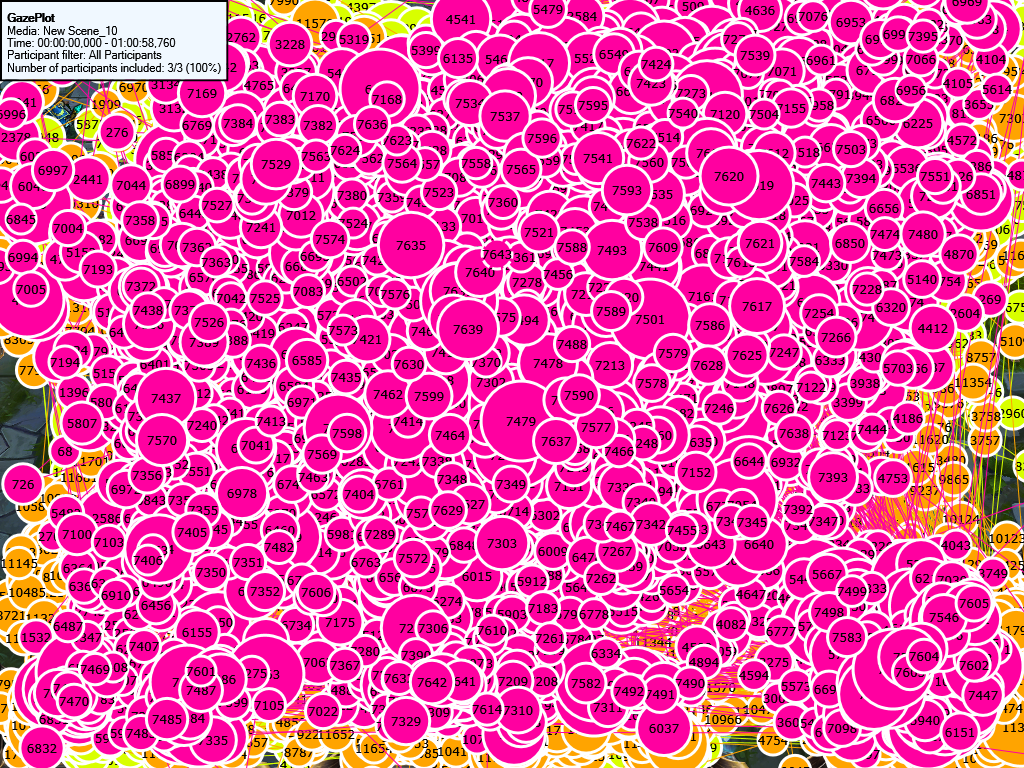
\includegraphics[width=\textwidth]{images/gazeplot/Noobs}
\caption{Gaze plot Group 1}
\label{gaze_noob}
\end{minipage}
\hspace{0.5cm}
\begin{minipage}[b]{0.45\linewidth}
\centering
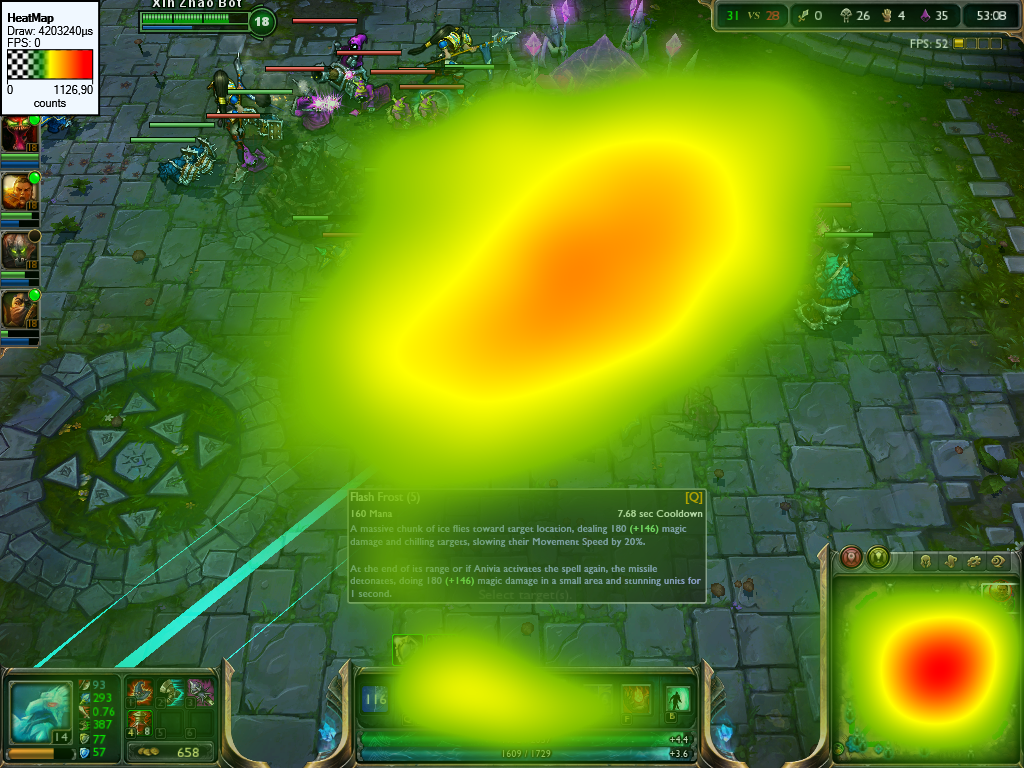
\includegraphics[width=\textwidth]{images/heatmap/Noobs}
\caption{Heat map Group 1}
\label{heat_noob}
\end{minipage}
\end{figure}

\begin{figure}[ht]
\begin{minipage}[b]{0.45\linewidth}
\centering
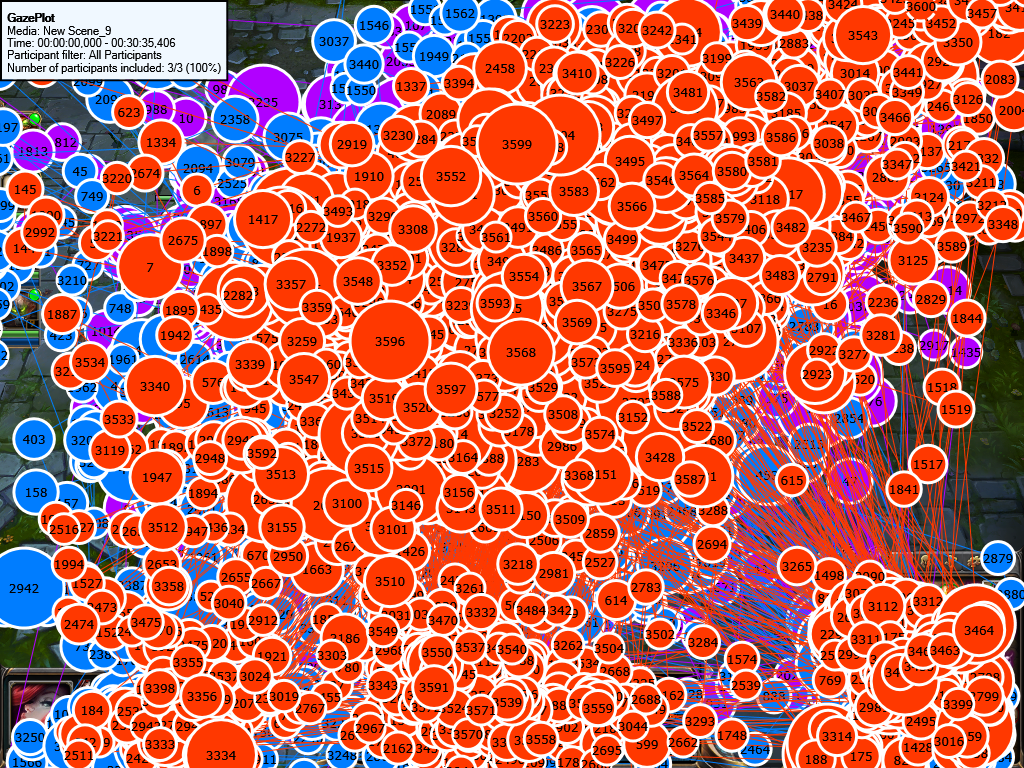
\includegraphics[width=\textwidth]{images/gazeplot/Pros}
\caption{Gaze plot Group 2}
\label{gaze_pro}
\end{minipage}
\hspace{0.5cm}
\begin{minipage}[b]{0.45\linewidth}
\centering
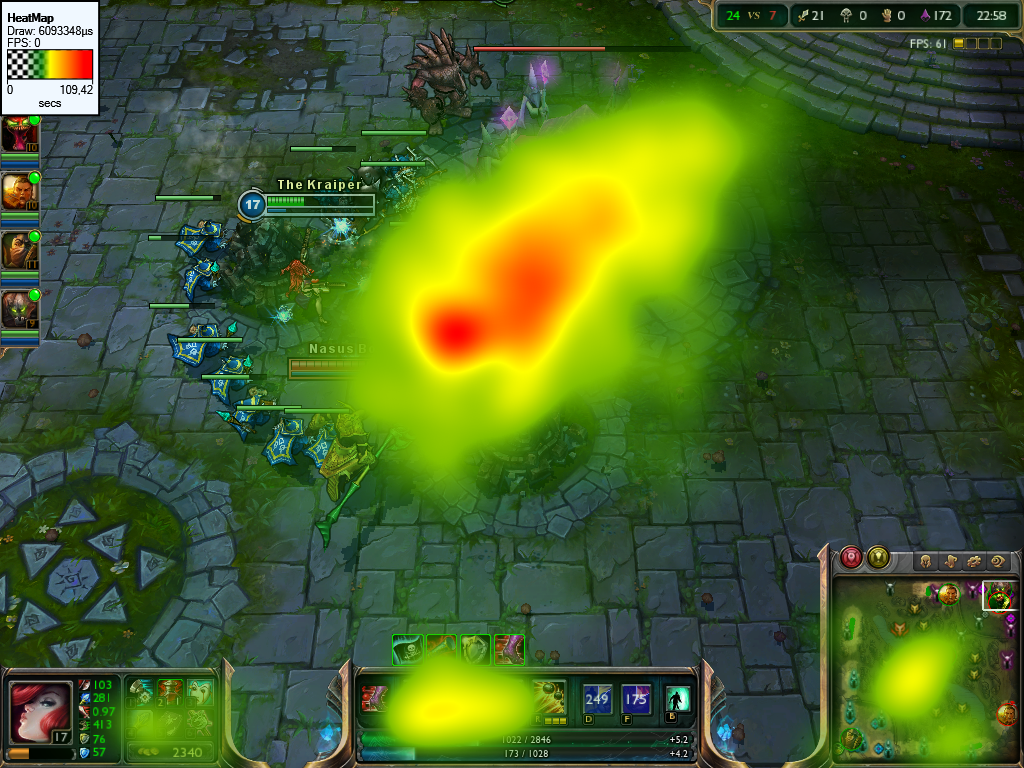
\includegraphics[width=\textwidth]{images/heatmap/Pros}
\caption{Heat map Group 2}
\label{heat_pro}
\end{minipage}
\end{figure}

\begin{figure}[ht]
\begin{minipage}[b]{0.45\linewidth}
\centering
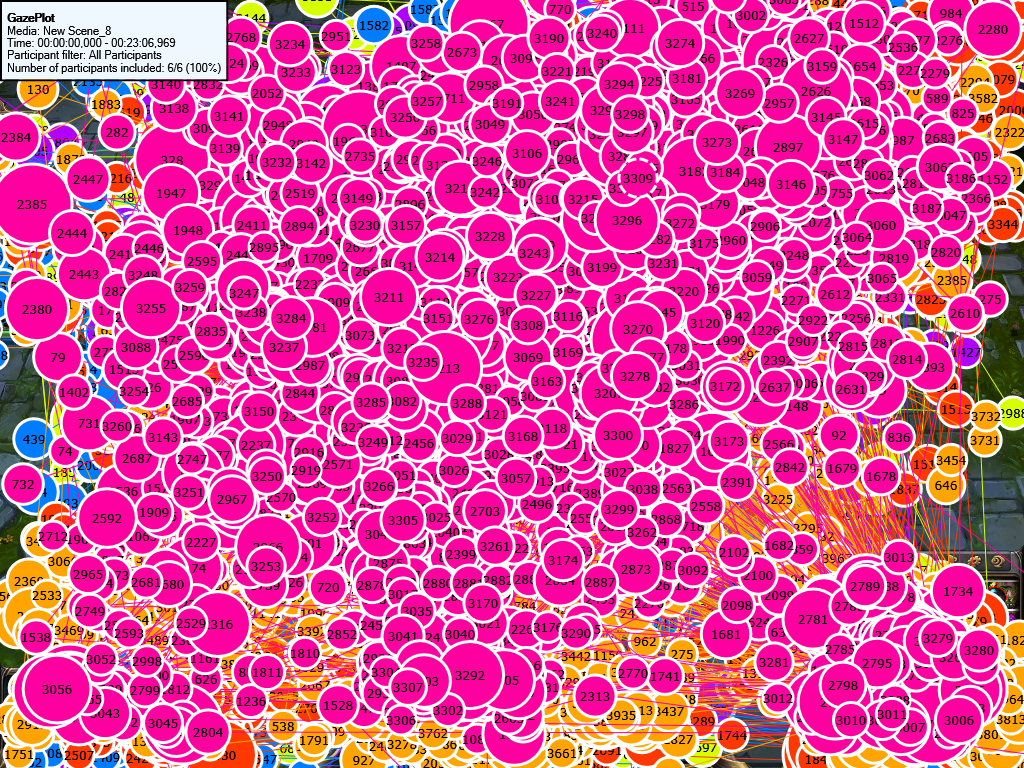
\includegraphics[width=\textwidth]{images/gazeplot/All}
\caption{Gaze plot all participants}
\label{gaze_all}
\end{minipage}
\hspace{0.5cm}
\begin{minipage}[b]{0.45\linewidth}
\centering
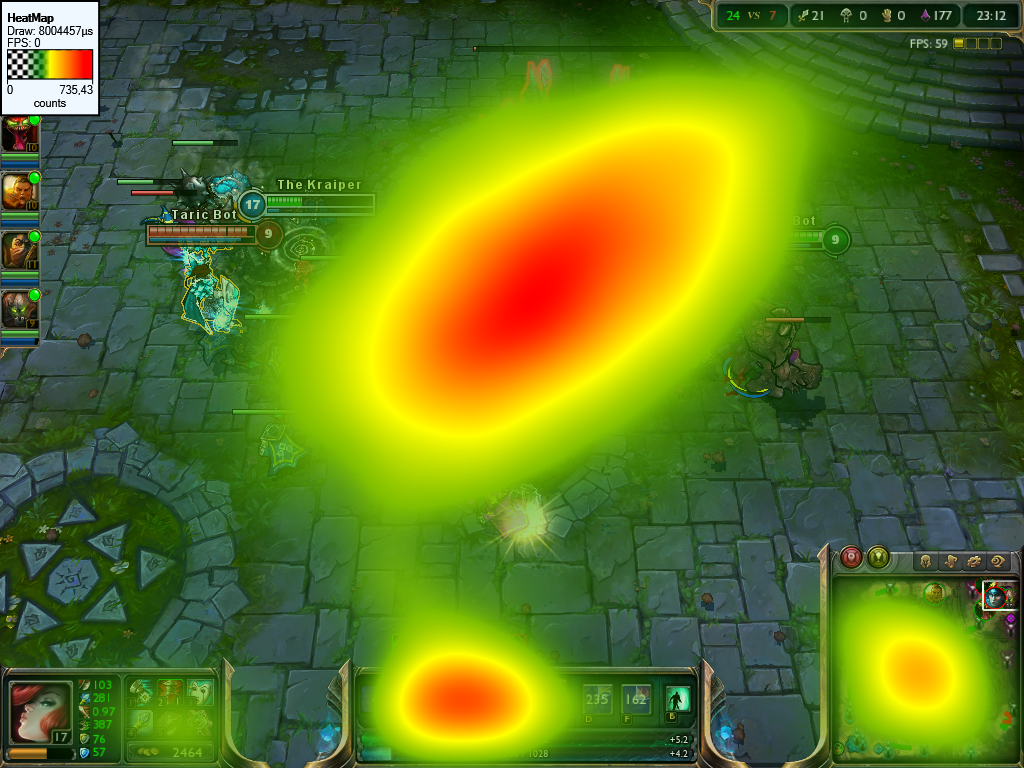
\includegraphics[width=\textwidth]{images/heatmap/All}
\caption{Heat map all participants}
\label{heat_all}
\end{minipage}
\end{figure}

\begin{figure}
\centering
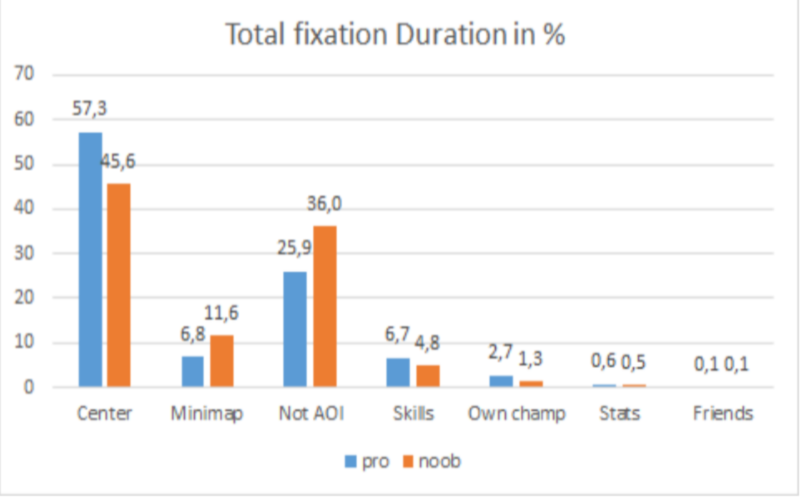
\includegraphics[width=0.8\textwidth]{images/AOIChart}
\caption{Graph showing the difference between how the two groups focus on areas of interest.}
\label{aoi_graph}
\end{figure}

\end{document}
